% Created 2020-06-23 mar. 19:34
% Intended LaTeX compiler: pdflatex
\documentclass{ISMA_USD2020}
\usepackage[utf8]{inputenc}
\usepackage[T1]{fontenc}
\usepackage{graphicx}
\usepackage{grffile}
\usepackage{longtable}
\usepackage{wrapfig}
\usepackage{rotating}
\usepackage[normalem]{ulem}
\usepackage{amsmath}
\usepackage{textcomp}
\usepackage{amssymb}
\usepackage{capt-of}
\usepackage{hyperref}
\usepackage[most]{tcolorbox}
\usepackage{bm}
\usepackage{booktabs}
\usepackage{tabularx}
\usepackage{array}
\usepackage{siunitx}
\usepackage{amsmath,amssymb,amsfonts, cases}
\usepackage{algorithmic, graphicx, textcomp}
\usepackage{xcolor, import, hyperref}
\usepackage[USenglish, english]{babel}
\setcounter{footnote}{1}
\usepackage[utf8]{inputenc}
\usepackage[T1]{fontenc}

\usepackage[french, english]{babel} % Last language is main language

\usepackage{lmodern} % Latin Modern Font
\usepackage{gensymb} % Generic symbols for both text and math mode

\usepackage{standalone} % Used to generate standalone Tikz

\usepackage{amsmath}   % Main math Package
\usepackage{mathtools} % Extension package to amsmath
\usepackage{amsthm}    % Typesetting theorems (AMS style)
\usepackage{amsfonts}  % More fonts from the AMS
\usepackage{textcomp}  % provide many text symbols
\usepackage{steinmetz} % For phase symbol

\usepackage{xstring}  % Utils to manipulate strings
\usepackage{etoolbox} % Add basic if/then
\usepackage{esvect}   % Beautyfull vectors
\usepackage{graphicx} % Enhanced support for graphics
\usepackage{grffile}  % Used by matlab2tikz

\usepackage{microtype} % typographic tuning
\usepackage{setspace}  % for line spacing, e.g. \onehalfspacing
\usepackage{tabularx}  % table features
\usepackage{enumitem}  % for simple list modifications
\usepackage{booktabs}  % better table support

\usepackage{stackengine} %

\usepackage[load-configurations=abbreviations]{siunitx} % SI units
\sisetup{
    locale = US,
    detect-all,
    range-phrase=--,
    range-units=single
}

\usepackage{tikz}       % Tikz
\usepackage{tikzscale}  % Used to scale Tikz graphics
\usepackage{adjustbox}  % Used to proper positioning of tikz pictures
\usepackage{circuitikz} % Draw electronic circuits
\usepackage{pgfpages}   % Needed to use notes
\usepackage{pgfplots}   % Used to plot functions

\usetikzlibrary{arrows}                   % Arrow tip library
\usetikzlibrary{arrows.meta}              % Add some arrows
\usetikzlibrary{calc}                     % The library allows advanced Coordinate Calculations
\usetikzlibrary{intersections}            % calculate intersections of paths
\usetikzlibrary{matrix}                   %
\usetikzlibrary{patterns}                 %
\usetikzlibrary{shapes}                   % Defines circle and rectangle
\usetikzlibrary{shapes.geometric}         % Use for the shape diamond and isosceles triangle
\usetikzlibrary{snakes}                   % snake=coil and snake=zigzag using segment amplitude=10pt
\usetikzlibrary{positioning}              % Additional options for placing nodes
\usetikzlibrary{3d}                       % Plot 3D shapes
\usetikzlibrary{spy}                      % Creating a magnified area
\usetikzlibrary{decorations.text}         % Used to make text follows a curve
\usetikzlibrary{decorations.pathmorphing} % deformation of a path
\usetikzlibrary{decorations.markings}     % Used for spring and damper
\usetikzlibrary{babel}                    % A tiny library that make the interaction with the babel package easier
\usetikzlibrary{plotmarks}                % This library defines a number of plot marks
\usetikzlibrary{fit}                      % Used to make rectangle as nodes by specifying two points
\usetikzlibrary{backgrounds}              % Used to put things under others

\usepgfplotslibrary{patchplots}
\usepgfplotslibrary{groupplots}

\pgfplotsset{compat=newest}
\pgfplotsset{plot coordinates/math parser=false}

\newlength{\fheight}
\newlength{\fwidth}

\setlength{\fwidth}{85mm}
\setlength{\fheight}{112mm}

\tikzset{>=Stealth}
% Setup default Linewidth
\tikzset{every path/.style={line width=1pt}}

\usepackage{xcolor}% Color extension

\definecolor{colorblack}{rgb}{0, 0, 0}
\definecolor{colorblue}{rgb}{0, 0.4470, 0.7410}
\definecolor{colorred}{rgb}{0.8500, 0.3250, 0.0980}
\definecolor{coloryellow}{rgb}{0.9290, 0.6940, 0.1250}
\definecolor{colorpurple}{rgb}{0.4940, 0.1840, 0.5560}
\definecolor{colorgreen}{rgb}{0.4660, 0.6740, 0.1880}
\definecolor{colorcyan}{rgb}{0.3010, 0.7450, 0.9330}
\definecolor{colorbordeau}{rgb}{0.6350, 0.0780, 0.1840}

% Main color
\definecolor{maincolor}{RGB}{89, 9, 38}
\definecolor{secondcolor}{RGB}{20, 9, 89}

\tikzset{%
  block/.style n args={2}{%
    draw,
    fill=white,
    minimum width  = #1,
    minimum height = #2,
  },
  block/.default={1.2cm}{1.0cm}
}

\tikzstyle{branch}=[fill,shape=circle,minimum size=4pt,inner sep=0pt]
\tikzstyle{->top}=[-{Stealth[color=black, scale=0.8]}, draw=white, double=black, double distance=1pt, line width=1pt]
\tikzstyle{<-top}=[{stealth[color=black, scale=0.8]}-, draw=white, double=black, double distance=1pt, line width=1pt]

\tikzstyle{handwriten}=[decorate,decoration={random steps,amplitude=0.1pt,segment length=0.8pt}]

\tikzset{%
  DAC/.style={%
    draw,
    signal,
  }
}

\tikzset{%
  ADC/.style={%
    draw,
    signal,
    signal to = west,
  }
}

\tikzset{%
  gain right/.style={%
    draw,
    regular polygon,
    regular polygon sides = 3,
    inner sep = 2pt,
    shape border rotate=-90
  },
  gain left/.style={%
    draw,
    regular polygon,
    regular polygon sides = 3,
    inner sep = 2pt,
    shape border rotate=90
  },
  gain top/.style={%
    draw,
    regular polygon,
    regular polygon sides = 3,
    inner sep = 2pt,
    shape border rotate=0
  },
  gain bottom/.style={%
    draw,
    regular polygon,
    regular polygon sides = 3,
    inner sep = 2pt,
    shape border rotate=180
  },
}

\tikzset{% Add block with Circled operations
  addc/.style n args={5}{%
    draw,
    fill=white,
    circle,
    outer sep = 0pt,
    inner sep = 0pt,
    minimum size = 2em,
    execute at begin node={\LARGE $#1$},
    append after command={\pgfextra{\let\mainnode=\tikzlastnode}
      \ifx#2\empty\else
      node[draw, circle, outer sep=6pt, inner sep=0pt, above left] at (\mainnode.west) {$#2$}%
      \fi
      \ifx#3\empty\else
      node[draw, circle, outer sep=6pt, inner sep=0pt, above right] at (\mainnode.north) {$#3$}%
      \fi
      \ifx#4\empty\else
      node[draw, circle, outer sep=6pt, inner sep=0pt, below right] at (\mainnode.east) {$#4$}%
      \fi
      \ifx#5\empty\else
      node[draw, circle, outer sep=6pt, inner sep=0pt, below left] at (\mainnode.south) {$#5$}%
      \fi
      }
  },
  addc/.default={+}{}{}{}{},
}

\tikzset{% Add Block
  addb/.style n args={5}{%
    draw,
    fill=white,
    circle,
    outer sep = 0pt,
    inner sep = 0pt,
    minimum size = 2em,
    execute at begin node={\LARGE $#1$},
    append after command={\pgfextra{\let\mainnode=\tikzlastnode}
      \ifx#2\empty\else
      node[outer sep=2pt, inner sep=0pt, above left] at (\mainnode.west) {$#2$}%
      \fi
      \ifx#3\empty\else
      node[outer sep=2pt, inner sep=0pt, above right] at (\mainnode.north) {$#3$}%
      \fi
      \ifx#4\empty\else
      node[outer sep=2pt, inner sep=0pt, below right] at (\mainnode.east) {$#4$}%
      \fi
      \ifx#5\empty\else
      node[outer sep=2pt, inner sep=0pt, below left] at (\mainnode.south) {$#5$}%
      \fi
      }
  },
  addb/.default={+}{}{}{}{},
}

\pgfplotsset{grid style={black}}
\pgfplotsset{major grid style={black!30!white}}
\pgfplotsset{minor grid style={black!10!white}}
\pgfplotsset{xmajorgrids}
\pgfplotsset{ymajorgrids}

\pgfplotsset{separate axis lines=false} % draw axis as rectangle and not as 4 lines
\pgfplotsset{every outer x axis line/.append style={black}}
\pgfplotsset{every outer y axis line/.append style={black}}
\pgfplotsset{axis background/.style={fill=white}}
\pgfplotsset{axis x line*=bottom} % solid line on the bottom with thin on the top
\pgfplotsset{axis y line*=left} % solid line on the left with thin on the right

\pgfplotsset{every y tick label/.append style={font=\color{black}}}
\pgfplotsset{every y tick/.append style={black}}
\pgfplotsset{every x tick label/.append style={font=\color{black}}}
\pgfplotsset{every x tick/.append style={black}}

\pgfplotsset{scale only axis=true}

\pgfplotsset{ylabel absolute}

% https://tex.stackexchange.com/questions/54794/using-a-pgfplots-style-legend-in-a-plain-old-tikzpicture#54834

% argument #1: any options
\newenvironment{customlegend}[1][]{%
  \begingroup
  % inits/clears the lists (which might be populated from previous
  % axes):
  \csname pgfplots@init@cleared@structures\endcsname
  \pgfplotsset{#1}%
}{%
  % draws the legend:
  \csname pgfplots@createlegend\endcsname
  \endgroup
}%

% makes \addlegendimage available (typically only available within an
% axis environment):
\def\addlegendimage{\csname pgfplots@addlegendimage\endcsname}

% definition to insert numbers
% \pgfkeys{/pgfplots/number in legend/.style={%
%     /pgfplots/legend image code/.code={%
%       \node at (0.125,-0.0225){#1}; % <= changed x value
%     },%
%   },
% }
\pgfplotsset{
  every legend to name picture/.style={west}
}

\tikzstyle{upperbound}=[line cap=round, postaction={decorate,draw,decoration={border, segment length=0.2cm, amplitude=0.3cm, angle=60}}]
\tikzstyle{lowerbound}=[line cap=round, postaction={decorate,draw,decoration={border, segment length=0.2cm, amplitude=0.3cm, angle=-60}}]

\pgfplotsset{
  /pgfplots/upperbound/.style 1 args={
    legend image code/.code={
      \draw[##1, upperbound]
        plot coordinates {
        (0cm,0cm)
        (0.6cm,0cm)
      }
    }
  }
}

\tikzset{%
  pole/.style{%
    color=red,
    cross out,
    draw,
    inner sep=0pt,
    outer sep=0pt,
    minimum size=#1pt
  },
  pole/.default={4}
}

\tikzset{%
  zero/.style{%
    color=red,
    circle,
    draw,
    inner sep=0pt,
    outer sep=0pt,
    minimum size=#1pt
  },
  zero/.default={4}
}

\tikzset{%
  spring/.style={%
    thick,
    decoration={
      zigzag,
      pre length  = #1cm,
      post length = #1cm,
      segment length = 6
    },
    decorate
  },
  spring/.default={0.2}
}

\tikzset{%
  coil/.style n args={2}{%
    thick,
    decoration={
      coil,
      pre length  = #1cm,
      post length = #2cm,
      segment length = 4
    },
    decorate
  },
  coil/.default={0.3}{0.3}
}

\tikzset{%
  damper/.style n args={2}{%
    thick,
    decoration={markings, mark connection node=dmp, mark=at position 0.5 with {
        \node (dmp) [thick,
                     inner sep = 0pt,
                     transform shape,
                     rotate  =-90,
                     minimum width  = #1pt,
                     minimum height = #2pt,
                     draw=none] {};
        \draw [thick] ($(dmp.north east)+(0.6*#2pt,0)$) -- (dmp.south east) -- (dmp.south west) -- ($(dmp.north west)+(0.6*#2pt,0)$);
        \draw [thick] ($(dmp.north)+(0,-0.3*#1pt)$) -- ($(dmp.north)+(0,0.3*#1pt)$);
      }
    },
    decorate
  },
  damper/.default={12}{3}
}

\tikzset{%
  actuator/.style n args={2}{%
    thick,
    draw=none,
    decoration={
      markings,
      mark connection node=my node,
      mark=at position .5 with {
        \node [draw, inner sep=0pt, minimum width=#1cm, minimum height=#2cm,
        transform shape, fill=white] (my node) {};
      },
      mark=at position .0 with {
        \draw[<-] (0, 0) -- (my node);
      },
      mark=at position 1.0 with {
        \draw[<-] (0, 0) -- (my node);
      }
    },
    decorate
  },
  actuator/.default={0.5}{0.2}
}

\tikzset{%
  ground/.style n args={2}{%
    fill,
    pattern = north east lines,
    draw = none,
    anchor = north,
    minimum width  = #1cm,
    minimum height = #2cm,
    append after command={
      (\tikzlastnode.north west) edge (\tikzlastnode.north east)
    }
  },
  ground/.default={2.5}{0.3}
}

\tikzset{%
  forcesensor/.style n args={2}{%
    rectangle,
    outer sep=0pt,
    inner sep=0pt,
    draw=black,
    fill=white!60!black,
    anchor=south,
    minimum width =#1cm,
    minimum height=#2cm,
    append after command={
      [every edge/.append style={
        thick,
        black,
      }]
      (\tikzlastnode.north west) edge (\tikzlastnode.south east)
      (\tikzlastnode.north east) edge (\tikzlastnode.south west)
    }
  },
  forcesensor/.default={2.0}{0.5}
}

\tikzset{%
  inertialsensor/.style={%
    rectangle,
    outer sep=0pt,
    inner sep=0pt,
    draw=black,
    fill=white!60!black,
    anchor=south east,
    minimum size=#1cm,
    append after command={
      [every edge/.append style={
        thick,
        black,
      }]
      (\tikzlastnode.north west) edge (\tikzlastnode.south east)
      (\tikzlastnode.north east) edge (\tikzlastnode.south west)
    }
  },
  inertialsensor/.default={0.3}
}

\newcommand{\AxisRotator}[1][rotate=0]{%
  \tikz [x=0.1cm,y=0.30cm,-stealth,#1] \draw (0,0) arc (-150:150:1 and 1);%
}

\tikzstyle{cross}=[path picture={
  \draw[black]
  (path picture bounding box.south east) -- (path picture bounding box.north west) (path picture bounding box.south west) -- (path picture bounding box.north east);
}]

\tikzset{%
  piezo/.style n args={3}{%
    draw,
    rectangle,
    minimum width  = #1cm,
    minimum height = #2cm,
    fill=blue!10!white,
    anchor=center,
    append after command={
      [every edge/.append style={
        thick,
        black,
      }]
      \foreach \i in {1,...,#3}{
        (${\i/(1+#3)}*(\tikzlastnode.north west)+{(1+#3-\i)/(1+#3)}*(\tikzlastnode.south west)+0.1*(#1,0)$) edge (${\i/(1+#3)}*(\tikzlastnode.north east)+{(1+#3-\i)/(1+#3)}*(\tikzlastnode.south east)-0.1*(#1,0)$)
      }
    }
  },
  piezo/.default={2}{4}{10}
}

\def\voicecoil#1#2#3{
  % ======================
  % Parameters
  % ======================
  \def\voicecoilw{#1} % Total Width
  \def\voicecoilh{#2} % Total Height

  \def\magnetw{\voicecoilw} % Width of the magnet
  \def\magneth{\voicecoilh/1.4} % Height of the magnet

  \def\magnetwb{0.15*\magnetw} % Width of the borders of the magnet
  \def\magnetmw{0.15*\magnetw} % Width of the middle part of the magnet
  \def\magnetwg{0.5*\magnetw} % Width of the gap of the magnet

  \def\magnethl{\magnetwb} % Height of the low part of the magnet
  \def\magnetmh{0.15*\magneth} % Height of the middle part of the magnet
  \def\magnethg{0.2*\magneth} % Height of the gap of the magnet
  % ======================

  \begin{scope}[shift={(0.5*\voicecoilw, 0.5*\voicecoilh)}, rotate=#3, shift={(0, -0.5*\voicecoilh)}]
    % ======================
    % Magnet
    % ======================
    \draw[fill=white] (0, 0) -| ++(0.5*\magnetw, \magneth) -| ++(-0.5*\magnetw+0.5*\magnetwg, -\magnethg) -| (0.5*\magnetw-\magnetwb, \magnethl) -| (-0.5*\magnetw+\magnetwb, \magneth-\magnethg) -| (-0.5*\magnetwg, \magneth) -| (-0.5*\magnetw, 0) -- (cycle);
    \begin{scope}[shift={(0, \magnethl)}]
      \draw[fill=red]  (-0.5*\magnetmw, 0) rectangle (0.5*\magnetmw, \magnetmh);
      \draw[fill=blue] (-0.5*\magnetmw, \magnetmh) rectangle (0.5*\magnetmw, 2*\magnetmh);
      % Top conductive Magnet
      \draw[fill=white] (-0.5*\magnetmw, 2*\magnetmh) -| (0.5*\magnetmw, -\magnethl+\magneth-\magnethg) -| ++(0.1, \magnethg) -| ++(-0.2-\magnetmw, -\magnethg) -| (-0.5*\magnetmw, \magnetmh);
    \end{scope}
    % ======================

    % ======================
    % Coil
    % ======================
    \pgfmathsetmacro{\coilwidth}{0.5*0.5*\magnetmw+0.5*0.1+0.25*\magnetwg}%
    \draw[] ( \coilwidth, 0.5*\magneth) -- ++(0, 0.7*\magneth);
    \draw[] (-\coilwidth, 0.5*\magneth) -- ++(0, 0.7*\magneth);
    % Point on the coil
    \foreach \x in {0,1,...,9}
    {
      \node[circle,inner sep=0.6pt,fill] at ( \coilwidth, \x*0.7*\magneth/10+0.5*\magneth);
      \node[circle,inner sep=0.6pt,fill] at (-\coilwidth, \x*0.7*\magneth/10+0.5*\magneth);
    }
    \draw[fill=white] (-0.5*\magnetw, 1.2*\magneth) rectangle ++(\magnetw, \magnethg);
    % ======================

    % ======================
    % Coordinates
    % ======================
    % Force
    \coordinate[] (vc_force) at (0, \magneth-0.5*\magnethg);
    % Coil
    \coordinate[] (vc_coil) at (0, \voicecoilh);
    % Magnet
    \coordinate[] (vc_magnet) at (0, 0);
    % Coil Wires
    \coordinate[] (vc_wire_one) at ( \coilwidth, 1.2*\magneth);
    \coordinate[] (vc_wire_two) at (-\coilwidth, 1.2*\magneth);
    % ======================
  \end{scope}
}

\tikzset{%
  ->-/.style={
    decoration={
      markings,
      mark = at position #1 with {\arrow{>}
      }
    },
    postaction={decorate}
  }
}
\tikzset{%
  -<-/.style={
    decoration={
      markings,
      mark = at position #1 with {\arrow{<}
      }
    },
    postaction={decorate}
  }
}

\tikzset{%
  labelc/.style= {%
    draw,
    fill=white,
    shape=circle,
    inner sep=2pt,
    outer sep=6pt,
  }
}

\author[1,3] {T. Dehaeze}
\author[1,2] {C. Collette}
\affil[1] {Precision Mechatronics Laboratory\NewLineAffil University of Liege, Belgium \NewAffil}
\affil[2] {BEAMS Department\NewLineAffil Free University of Brussels, Belgium \NewAffil}
\affil[3] {European Synchrotron Radiation Facility \NewLineAffil Grenoble, France e-mail: \textbf{thomas.dehaeze@esrf.fr}}
\bibliographystyle{IEEEtran}
\usepackage{tikz}
\usetikzlibrary{shapes.misc}
\date{}
\title{Active Damping of Rotating Positioning Platforms}
\hypersetup{
 pdfauthor={},
 pdftitle={Active Damping of Rotating Positioning Platforms},
 pdfkeywords={},
 pdfsubject={},
 pdfcreator={Emacs 27.0.91 (Org mode 9.4)}, 
 pdflang={English}}
\begin{document}

\maketitle

\abstract{
    Abstract text to be done
}

\section{Introduction}
\label{sec:org977317c}
\label{sec:introduction}
Controller Poles are shown by black crosses (
\begin{tikzpicture} \node[cross out, draw=black, minimum size=1ex, line width=2pt, inner sep=0pt, outer sep=0pt] at (0, 0){}; \end{tikzpicture}
).
\cite{dehaeze18_sampl_stabil_for_tomog_exper}

\section{System Under Study}
\label{sec:org042e800}
\subsection{Rotating Positioning Platform}
\label{sec:org489e4b9}
Consider the rotating X-Y stage of Figure \ref{fig:rotating_xy_platform}.

\begin{itemize}
\item \(k\): Actuator's Stiffness [N/m]
\item \(m\): Payload's mass [kg]
\item \(\Omega = \dot{\theta}\): rotation speed [rad/s]
\item \(F_u\), \(F_v\)
\item \(d_u\), \(d_v\)
\end{itemize}

\begin{figure}[htbp]
\centering
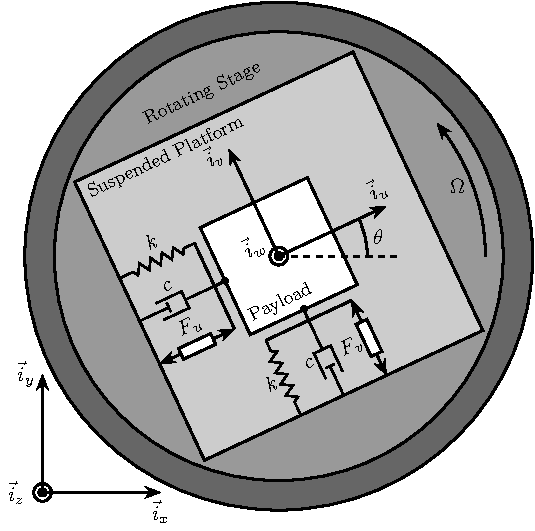
\includegraphics[scale=1]{figs/system.pdf}
\caption{\label{fig:rotating_xy_platform}Figure caption}
\end{figure}


\begin{figure}[htbp]
\centering
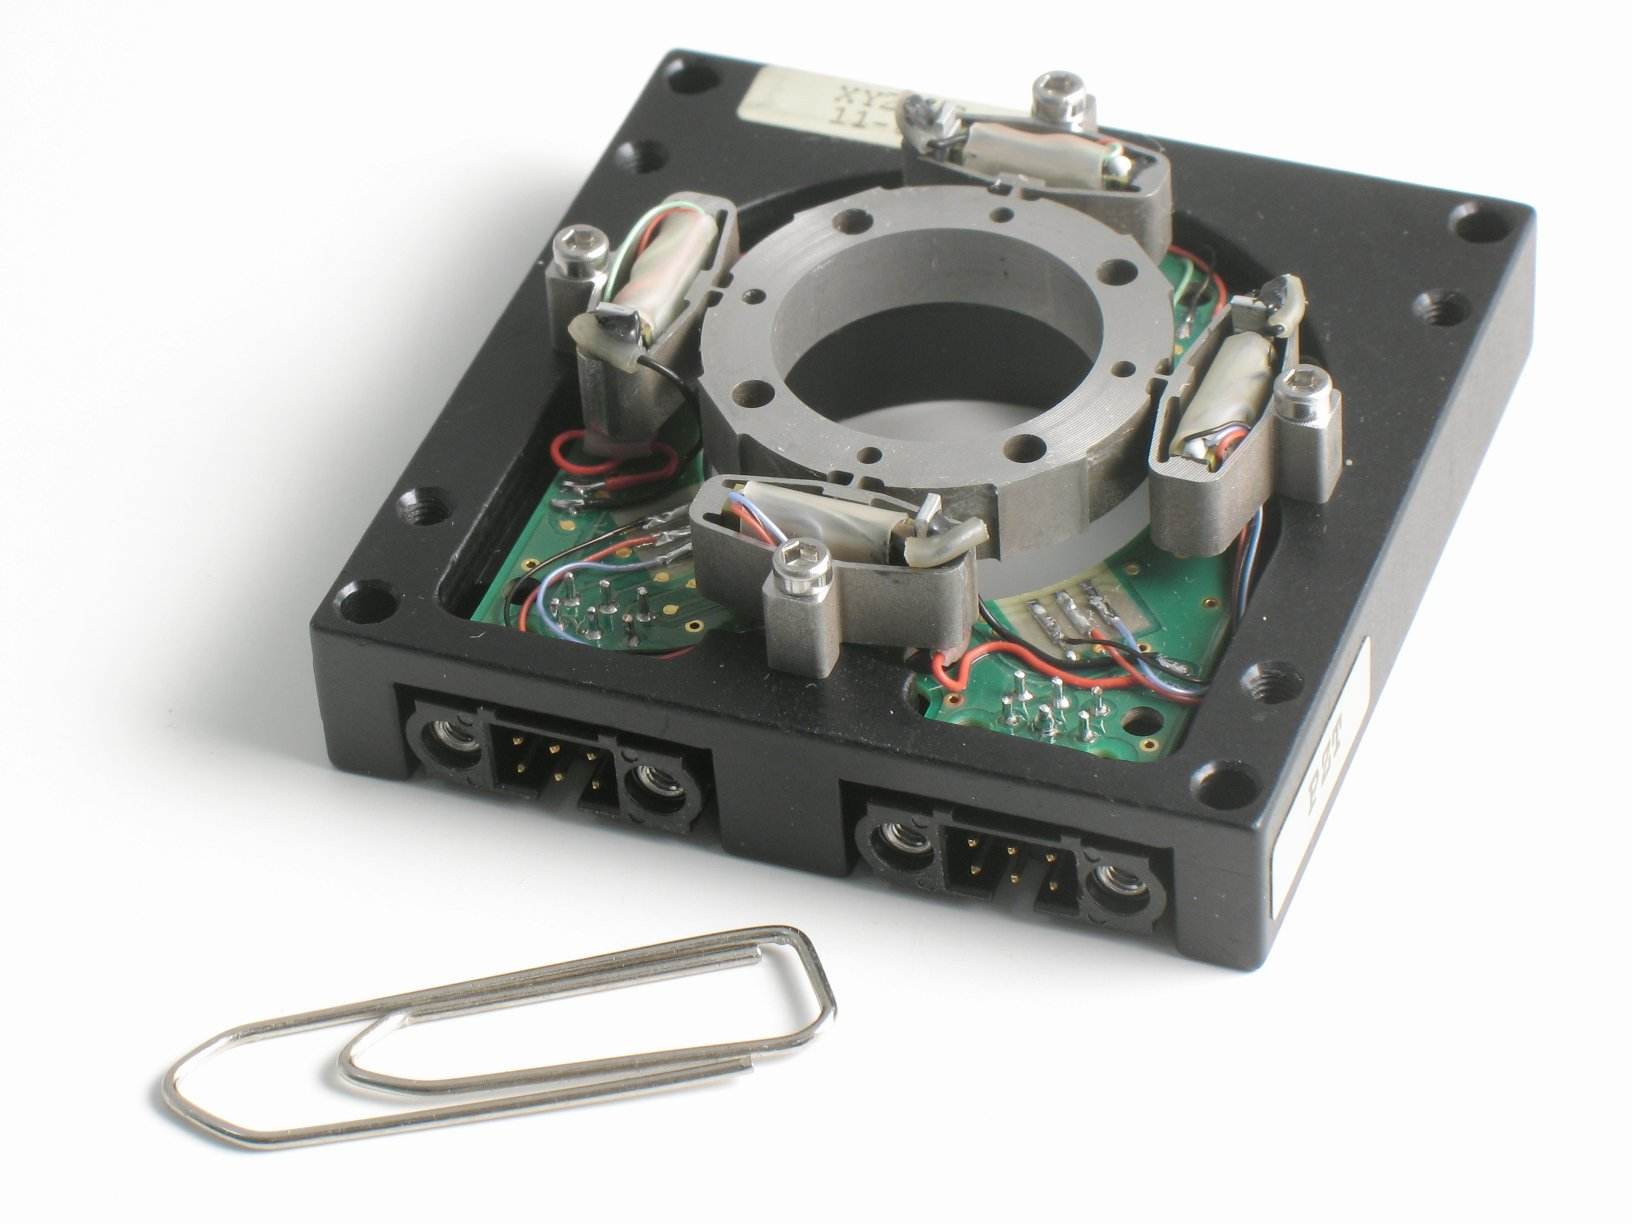
\includegraphics[width=0.5\linewidth]{figs/cedrat_xy25xs.jpg}
\caption{\label{fig:cedrat_xy25xs}Figure caption}
\end{figure}

\subsection{Equation of Motion}
\label{sec:orgb1836d5}
The system has two degrees of freedom and is thus fully described by the generalized coordinates \(u\) and \(v\).

Let's express the kinetic energy \(T\) and the potential energy \(V\) of the mass \(m\) (neglecting the rotational energy):

Dissipation function \(R\)
Kinetic energy \(T\)
Potential energy \(V\)
\begin{subequations}
  \begin{align}
    T & = \frac{1}{2} m \left( \left( \dot{u} - \Omega v \right)^2 + \left( \dot{v} + \Omega u \right)^2 \right) \\
    R & = \frac{1}{2} c \left( \dot{u}^2 + \dot{v}^2 \right) \\
    V & = \frac{1}{2} k \left( u^2 + v^2 \right)
  \end{align}
\end{subequations}

The Lagrangian is the kinetic energy minus the potential energy:
\begin{equation}
L = T - V
\end{equation}

From the Lagrange's equations of the second kind, the equation of motion is obtained (\(q_1 = u\), \(q_2 = v\)).
\begin{equation}
  \frac{d}{dt} \left( \frac{\partial L}{\partial \dot{q}_i} \right) + \frac{\partial D}{\partial \dot{q}_i} - \frac{\partial L}{\partial q_i} = Q_i
\end{equation}
with \(Q_i\) is the generalized force associated with the generalized variable \(q_i\) (\(Q_1 = F_u\) and \(Q_2 = F_v\)).


\begin{subequations}
  \begin{align}
    m \ddot{u} + c \dot{u} + ( k - m \Omega ) u &= F_u + 2 m \Omega \dot{v} \\
    m \ddot{v} + c \dot{v} + ( k \underbrace{-\,m \Omega}_{\text{Centrif.}} ) v &= F_v \underbrace{-\,2 m \Omega \dot{u}}_{\text{Coriolis}}
  \end{align}
\end{subequations}

\begin{itemize}
\item Coriolis Forces: coupling
\item Centrifugal forces: negative stiffness
\end{itemize}

Without the coupling terms, each equation is the equation of a one degree of freedom mass-spring system with mass \(m\) and stiffness \(k- m\dot{\theta}^2\).
Thus, the term \(- m\dot{\theta}^2\) acts like a negative stiffness (due to \textbf{centrifugal forces}).


\subsection{Transfer Functions in the Laplace domain}
\label{sec:orgb1002ed}

\begin{subequations}
  \begin{align}
    u &= \frac{ms^2 + cs + k - m \Omega^2}{\left( m s^2 + cs + k - m \Omega^2 \right)^2 + \left( 2 m \Omega s \right)^2} F_u +  \frac{2 m \Omega s}{\left( m s^2 + cs + k - m \Omega^2 \right)^2 + \left( 2 m \Omega s \right)^2} F_v \\
    v &= \frac{-2 m \Omega s}{\left( m s^2 + cs + k - m \Omega^2 \right)^2 + \left( 2 m \Omega s \right)^2} F_u +  \frac{ms^2 + cs + k - m \Omega^2}{\left( m s^2 + cs + k - m \Omega^2 \right)^2 + \left( 2 m \Omega s \right)^2} F_v
  \end{align}
\end{subequations}

\begin{equation}
\begin{bmatrix} d_u \\ d_v \end{bmatrix} =
\bm{G}_d
\begin{bmatrix} F_u \\ F_v \end{bmatrix}
\end{equation}
Where \(\bm{G}_d\) is a \(2 \times 2\) transfer function matrix.

\begin{equation}
\bm{G}_d = \frac{1}{k} \frac{1}{G_{dp}}
\begin{bmatrix}
   G_{dz} & G_{dc} \\
  -G_{dc} & G_{dz}
\end{bmatrix}
\end{equation}
With:
\begin{subequations}
  \begin{align}
    G_{dp} &= \left( \frac{s^2}{{\omega_0}^2} + 2 \xi \frac{s}{\omega_0} + 1 - \frac{{\Omega}^2}{{\omega_0}^2} \right)^2 + \left( 2 \frac{\Omega}{\omega_0} \frac{s}{\omega_0} \right)^2 \\
    G_{dz} &= \frac{s^2}{{\omega_0}^2} + 2 \xi \frac{s}{\omega_0} + 1 - \frac{{\Omega}^2}{{\omega_0}^2} \\
    G_{dc} &= 2 \frac{\Omega}{\omega_0} \frac{s}{\omega_0}
  \end{align}
\end{subequations}

\begin{itemize}
\item \(\omega_0 = \sqrt{\frac{k}{m}}\): Natural frequency of the mass-spring system in \(\si{\radian/\s}\)
\item \(\xi\) damping ratio
\end{itemize}


\subsection{Constant Rotating Speed}
\label{sec:orga4faf60}
To simplify, let's consider a constant rotating speed \(\dot{\theta} = \Omega\) and thus \(\ddot{\theta} = 0\).

\begin{equation}
\label{eq:coupledplant}
\begin{bmatrix} d_u \\ d_v \end{bmatrix} =
\frac{1}{(m s^2 + (k - m{\omega_0}^2))^2 + (2 m {\omega_0} s)^2}
\begin{bmatrix}
  ms^2 + (k-m{\omega_0}^2) & 2 m \omega_0 s \\
  -2 m \omega_0 s          & ms^2 + (k-m{\omega_0}^2) \\
\end{bmatrix}
\begin{bmatrix} F_u \\ F_v \end{bmatrix}
\end{equation}

\begin{equation}
\label{eq:coupled_plant}
\begin{bmatrix} d_u \\ d_v \end{bmatrix} =
\frac{\frac{1}{k}}{\left( \frac{s^2}{{\omega_0}^2} + (1 - \frac{{\Omega}^2}{{\omega_0}^2}) \right)^2 + \left( 2 \frac{{\Omega} s}{{\omega_0}^2} \right)^2}
\begin{bmatrix}
  \frac{s^2}{{\omega_0}^2} + 1 - \frac{{\Omega}^2}{{\omega_0}^2} & 2 \frac{\Omega s}{{\omega_0}^2} \\
  -2 \frac{\Omega s}{{\omega_0}^2}          & \frac{s^2}{{\omega_0}^2} + 1 - \frac{{\Omega}^2}{{\omega_0}^2} \\
\end{bmatrix}
\begin{bmatrix} F_u \\ F_v \end{bmatrix}
\end{equation}

When the rotation speed is null, the coupling terms are equal to zero and the diagonal terms corresponds to one degree of freedom mass spring system.
\begin{equation}
\label{eq:coupled_plant_no_rot}
\begin{bmatrix} d_u \\ d_v \end{bmatrix} =
\frac{\frac{1}{k}}{\frac{s^2}{{\omega_0}^2} + 1}
\begin{bmatrix}
  1 & 0 \\
  0 & 1
\end{bmatrix}
\begin{bmatrix} F_u \\ F_v \end{bmatrix}
\end{equation}

When the rotation speed in not null, the resonance frequency is duplicated into two pairs of complex conjugate poles.
As the rotation speed increases, one of the two resonant frequency goes to lower frequencies as the other one goes to higher frequencies (Figure \ref{fig:campbell_diagram}).

\begin{figure}[htbp]
\centering
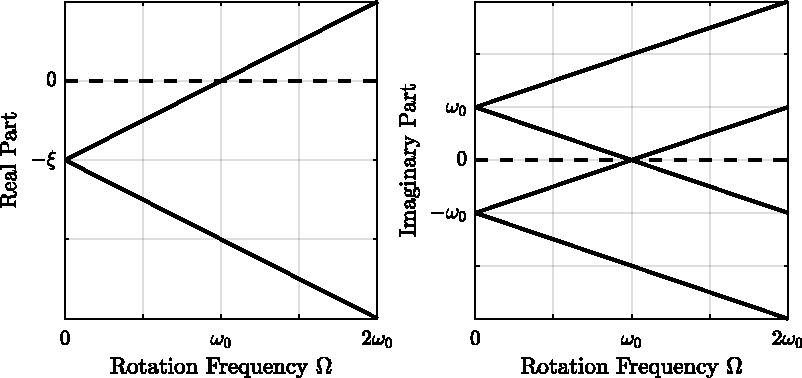
\includegraphics[scale=1]{figs/campbell_diagram.pdf}
\caption{\label{fig:campbell_diagram}Campbell Diagram}
\end{figure}

The magnitude of the coupling terms are increasing with the rotation speed.

\begin{figure}[htbp]
\centering
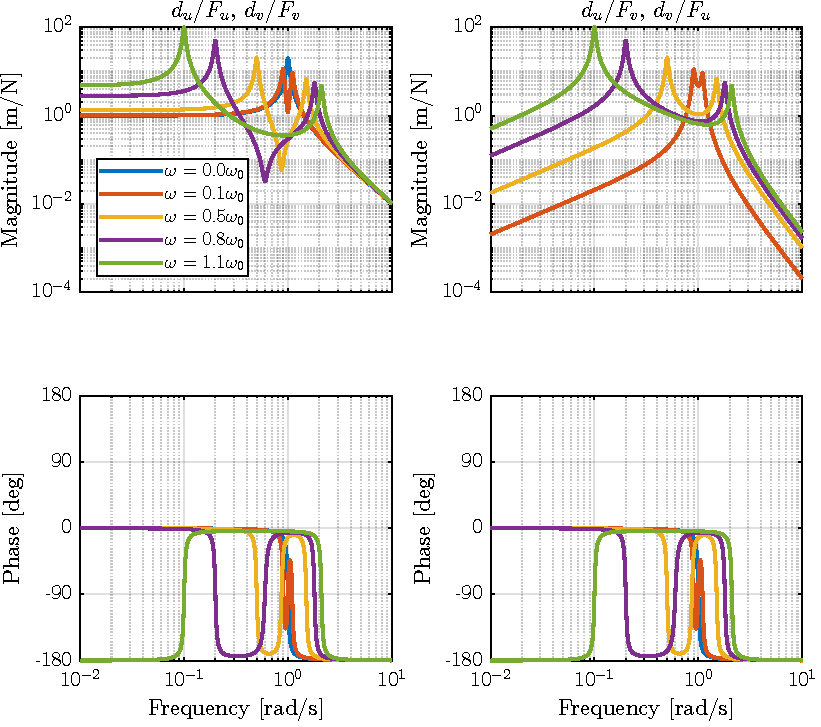
\includegraphics[scale=1]{figs/plant_compare_rotating_speed.pdf}
\caption{\label{fig:plant_compare_rotating_speed}Caption}
\end{figure}

\section{Integral Force Feedback}
\label{sec:orgaf500b0}
\subsection{Control Schematic}
\label{sec:orgbd9f859}

Force Sensors are added in series with the actuators as shown in Figure \ref{fig:system_iff}.

\begin{figure}[htbp]
\centering
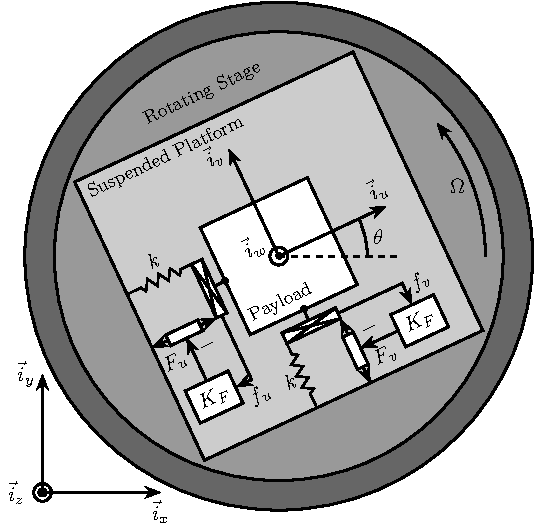
\includegraphics[scale=1]{figs/system_iff.pdf}
\caption{\label{fig:system_iff}System with Force Sensors in Series with the Actuators. Decentralized Integral Force Feedback is used}
\end{figure}

\subsection{Equations}
\label{sec:org48206d5}
The sensed forces are equal to:
\begin{equation}
\begin{bmatrix} f_{u} \\ f_{v} \end{bmatrix} =
\begin{bmatrix} F_u \\ F_v \end{bmatrix} - (c s + k)
\begin{bmatrix} d_u \\ d_v \end{bmatrix}
\end{equation}

Which then gives:
\begin{equation}
\begin{bmatrix} f_{u} \\ f_{v} \end{bmatrix} =
\bm{G}_{f}
\begin{bmatrix} F_u \\ F_v \end{bmatrix}
\end{equation}

\begin{equation}
\begin{bmatrix} f_{u} \\ f_{v} \end{bmatrix} =
\frac{1}{G_{fp}}
\begin{bmatrix}
  G_{fz} & -G_{fc} \\
  G_{fc} &  G_{fz}
\end{bmatrix}
\begin{bmatrix} F_u \\ F_v \end{bmatrix}
\end{equation}

\begin{align}
  G_{fp} &= \left( \frac{s^2}{{\omega_0}^2} + 2 \xi \frac{s}{\omega_0} + 1 - \frac{{\Omega}^2}{{\omega_0}^2} \right)^2 + \left( 2 \frac{\Omega}{\omega_0} \frac{s}{\omega_0} \right)^2 \\
  G_{fz} &= \left( \frac{s^2}{{\omega_0}^2} - \frac{\Omega^2}{{\omega_0}^2} \right) \left( \frac{s^2}{{\omega_0}^2} + 2 \xi \frac{s}{\omega_0} + 1 - \frac{{\Omega}^2}{{\omega_0}^2} \right) + \left( 2 \frac{\Omega}{\omega_0} \frac{s}{\omega_0} \right)^2 \\
  G_{fc} &= \left( 2 \xi \frac{s}{\omega_0} + 1 \right) \left( 2 \frac{\Omega}{\omega_0} \frac{s}{\omega_0} \right)
\end{align}


\subsection{Plant Dynamics}
\label{sec:orgec8431d}

\begin{figure}[htbp]
\centering
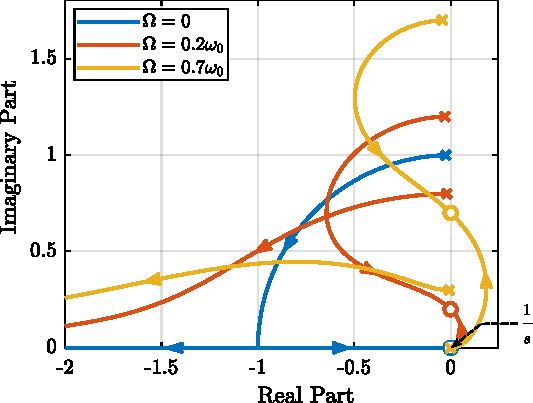
\includegraphics[scale=1]{figs/root_locus_pure_iff.pdf}
\caption{\label{fig:root_locus_pure_iff}Root Locus}
\end{figure}

\subsection{Physical Interpretation}
\label{sec:org159680e}

At low frequency, the gain is very large and thus no force is transmitted between the payload and the rotating stage.
This means that at low frequency, the system is decoupled (the force sensor removed) and thus the system is unstable.

\section{Integral Force Feedback with High Pass Filters}
\label{sec:org694707d}
\subsection{Modification of the Control Low}
\label{sec:org931fb10}

\subsection{Close Loop Analysis}
\label{sec:org9de0aa7}

\begin{figure}[htbp]
\centering
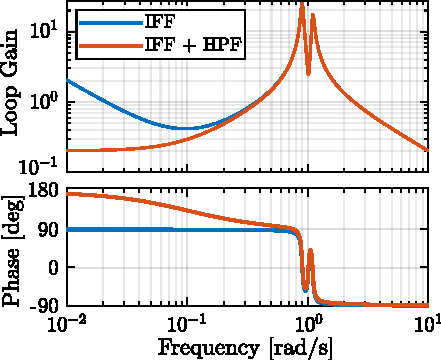
\includegraphics[scale=1]{figs/loop_gain_modified_iff.pdf}
\caption{\label{fig:loop_gain_modified_iff}Figure caption}
\end{figure}

\begin{figure}[htbp]
\centering
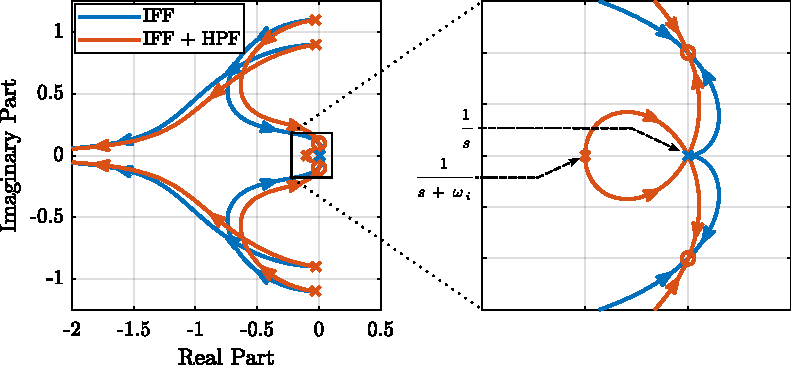
\includegraphics[scale=1]{figs/root_locus_modified_iff_ter.pdf}
\caption{\label{fig:root_locus_modified_iff}Figure caption}
\end{figure}

\subsection{Optimal Cut-Off Frequency}
\label{sec:org9808de1}

\begin{figure}[htbp]
\centering
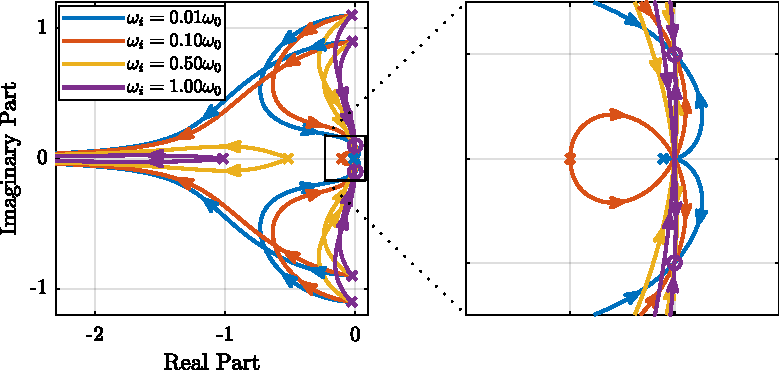
\includegraphics[scale=1]{figs/root_locus_wi_modified_iff_bis.pdf}
\caption{\label{fig:root_locus_wi_modified_iff}Figure caption}
\end{figure}


\begin{figure}[htbp]
\centering
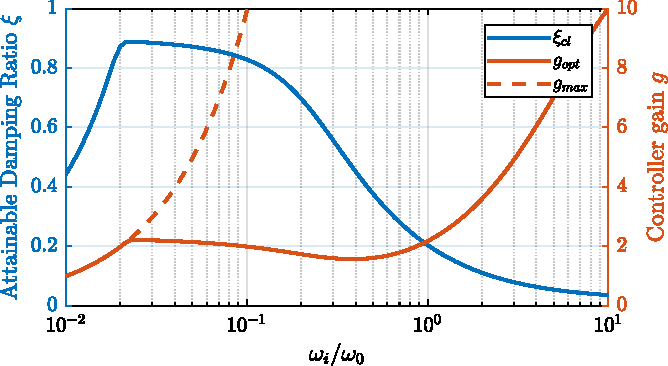
\includegraphics[scale=1]{figs/mod_iff_damping_wi.pdf}
\caption{\label{fig:mod_iff_damping_wi}Figure caption}
\end{figure}

\section{Integral Force Feedback with Parallel Springs}
\label{sec:orgd4915d5}

\begin{figure}[htbp]
\centering
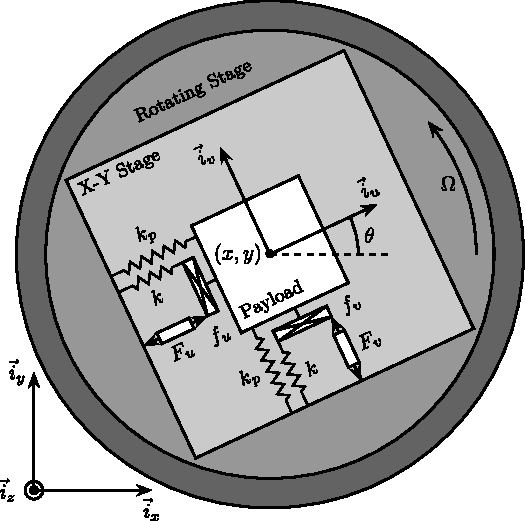
\includegraphics[scale=1]{figs/rotating_xy_platform_springs.pdf}
\caption{\label{fig:rotating_xy_platform_springs}Figure caption}
\end{figure}

\begin{figure}[htbp]
\centering
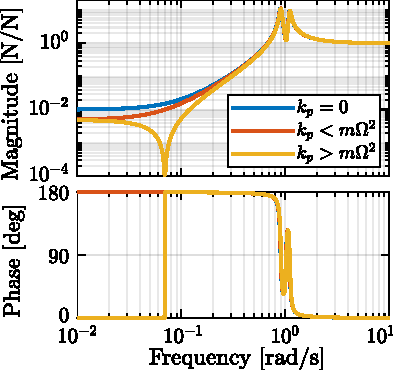
\includegraphics[scale=1]{figs/plant_iff_kp.pdf}
\caption{\label{fig:plant_iff_kp}Figure caption}
\end{figure}

\begin{figure}[htbp]
\centering
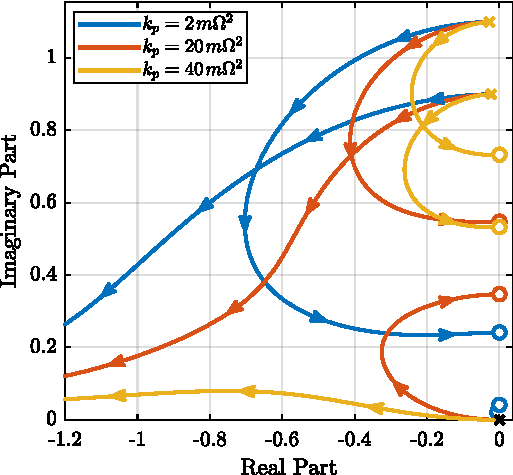
\includegraphics[scale=1]{figs/root_locus_iff_kps.pdf}
\caption{\label{fig:root_locus_iff_kps}Figure caption}
\end{figure}

\begin{figure}[htbp]
\centering
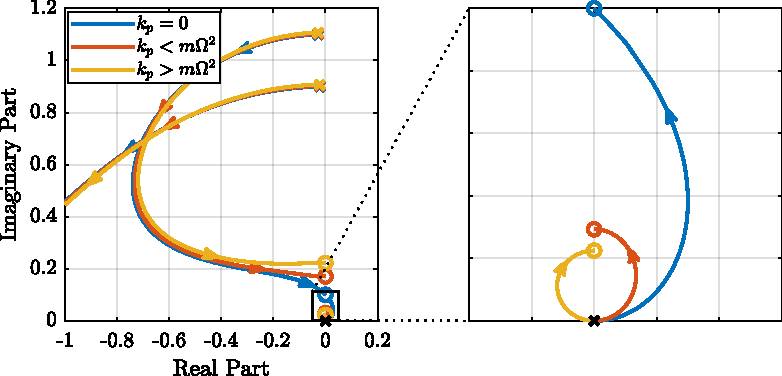
\includegraphics[scale=1]{figs/root_locus_iff_kp_ter.pdf}
\caption{\label{fig:root_locus_iff_kp_bis}Figure caption}
\end{figure}

\begin{figure}[htbp]
\centering
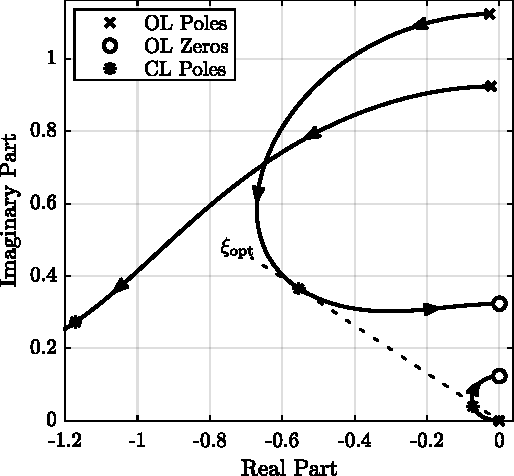
\includegraphics[scale=1]{figs/root_locus_opt_gain_iff_kp.pdf}
\caption{\label{fig:root_locus_opt_gain_iff_kp}Figure caption}
\end{figure}

\begin{figure}[htbp]
\centering
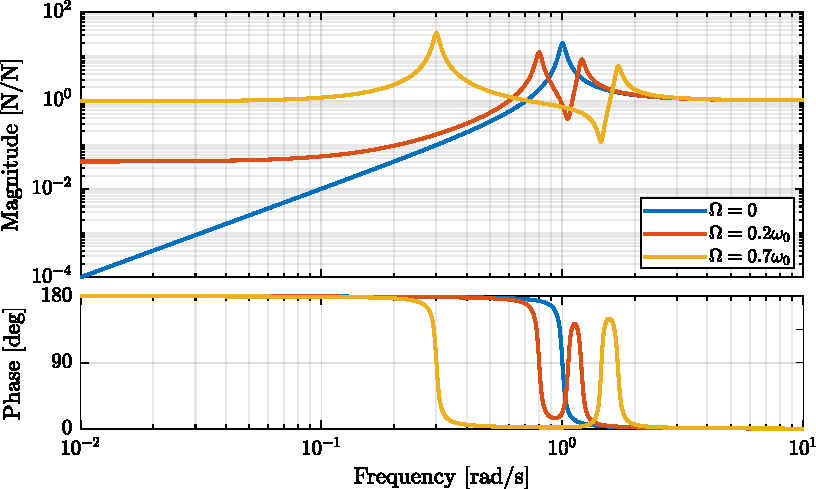
\includegraphics[scale=1]{figs/plant_iff_compare_rotating_speed.pdf}
\caption{\label{fig:plant_iff_compare_rotating_speed}Figure caption}
\end{figure}

\section{Direct Velocity Feedback}
\label{sec:orgb0a5870}

\begin{figure}[htbp]
\centering
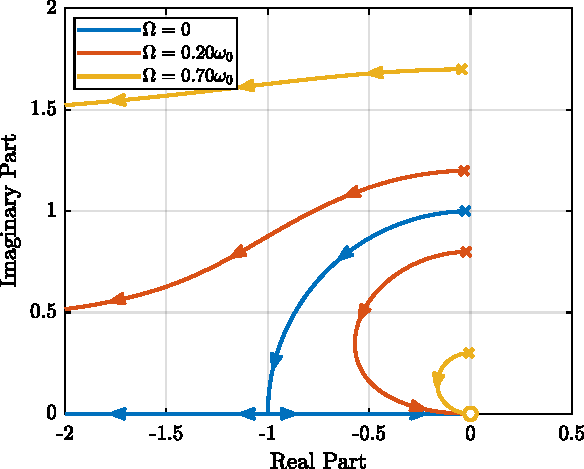
\includegraphics[scale=1]{figs/root_locus_dvf.pdf}
\caption{\label{fig:root_locus_dvf}Figure caption}
\end{figure}

\section{Comparison of the Proposed Active Damping Techniques}
\label{sec:org6097c1d}

\begin{figure}[htbp]
\centering
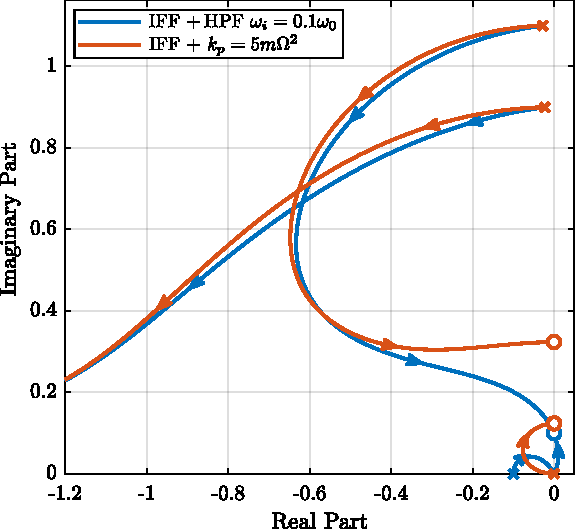
\includegraphics[scale=1]{figs/comp_root_locus.pdf}
\caption{\label{fig:comp_root_locus}Figure caption}
\end{figure}

\begin{figure}[htbp]
\centering
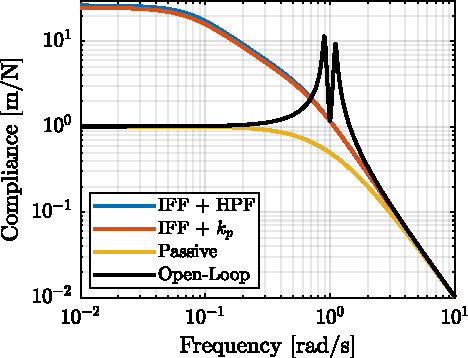
\includegraphics[scale=1]{figs/comp_compliance.pdf}
\caption{\label{fig:comp_compliance}Figure caption}
\end{figure}

\begin{figure}[htbp]
\centering
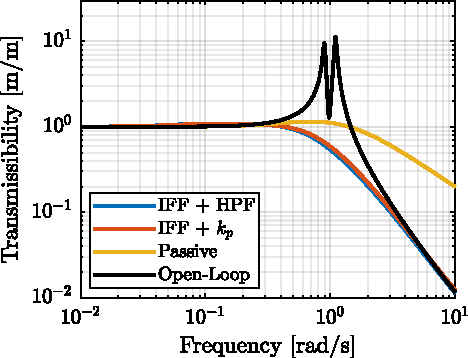
\includegraphics[scale=1]{figs/comp_transmissibility.pdf}
\caption{\label{fig:comp_transmissibility}Figure caption}
\end{figure}

\section{Conclusion}
\label{sec:org1624a6b}
\label{sec:conclusion}


\section*{Acknowledgment}
\label{sec:org1b29790}

\bibliography{ref.bib}
\end{document}
